\section{Руководство пользователя}
Результаты работы части функционала информационной системы представлены на скрин-шотах ниже. 


\begin{figure}[b!]
    \centering
    \begin{tabular}{cccc}
         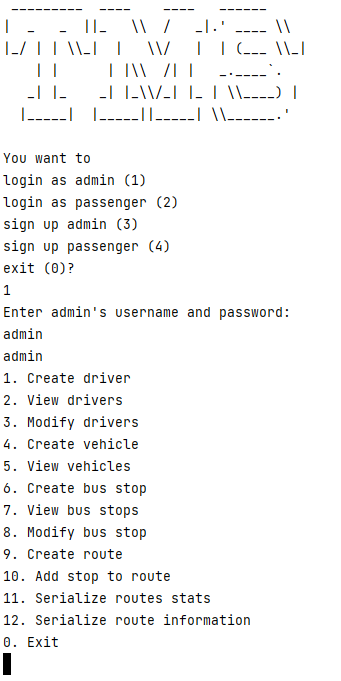
\includegraphics[height=9cm]{images/Login_Admin.png} & 
         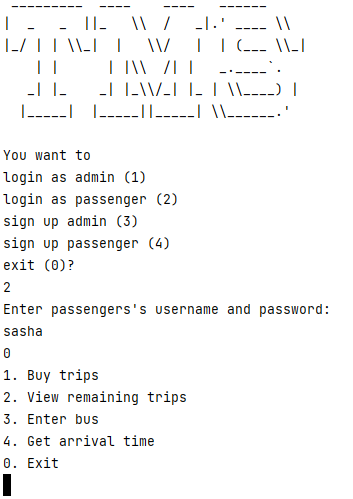
\includegraphics[height=9cm]{images/Login_Passenger.png} \\
         а & б \\[1em]
    \end{tabular}
    \caption{Процесс аутентификации а - администратора, б - пассажира}
\end{figure}

\begin{figure}[b!!]
    \centering
    \begin{tabular}{cccc}
         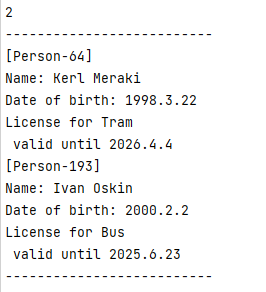
\includegraphics[width=7.5cm]{images/ViewDrivers.png} & 
         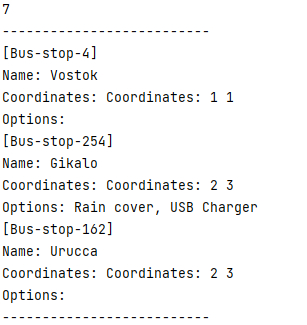
\includegraphics[width=7.5cm]{images/ViewStops.png}  \\
         а & б \\[1em]
    \end{tabular}
        \begin{tabular}{cccc}
         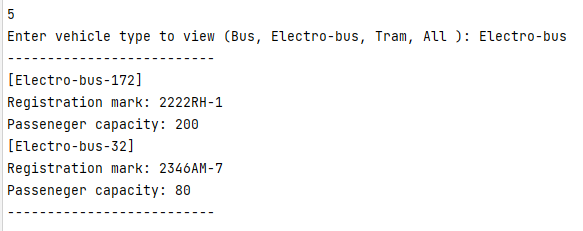
\includegraphics[width=7.5cm]{images/ViewVehicles.png} &
         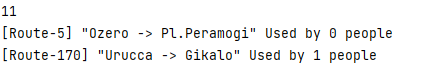
\includegraphics[width=7.5cm]{images/ViewStats.png} \\
         в & г\\[1em]
    \end{tabular}
    \caption{Просмотр существующих а - водителей, б - остановок, в - транспортных средств, г - статистики машрутов}
\end{figure}


\begin{figure}
    \centering
    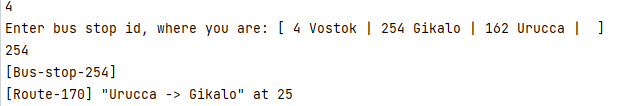
\includegraphics[scale=0.95]{images/ViewTimeTable.png}
    \caption{Просмотр расписания на остановке}
\end{figure}

\begin{figure}
    \centering
    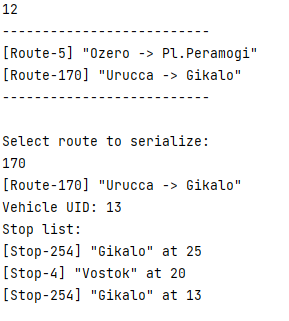
\includegraphics{images/RouteSerialize.png}
    \caption{Просмотр выбранного маршрута}
\end{figure}

\begin{figure}
    \centering
    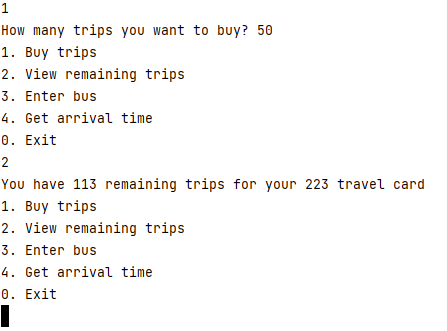
\includegraphics{images/Increment_Trips.png}
    \caption{Пополнение проездного}
\end{figure}

\begin{figure}
    \centering
    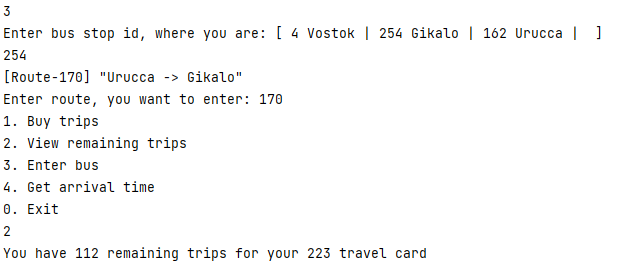
\includegraphics{images/EnterBus_decrement.png}
    \caption{Вход в ТС на остановке и уменьшение количества поездок}
\end{figure}

\begin{figure}
    \centering
    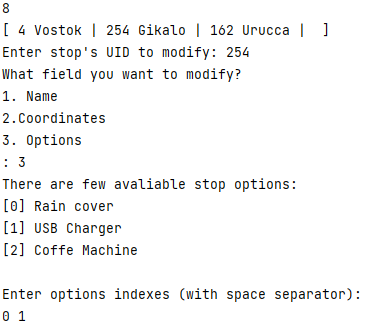
\includegraphics{images/BusStopEdit.png}
    \caption{Редактирование остановки}
\end{figure}